\documentclass[a4paper]{article}
\usepackage[normalem]{ulem}
\usepackage{eurosym}
\usepackage[font=small,labelfont=bf]{caption}

% impostazioni generali
%Tutti gli usepackage vanno qui
\usepackage{geometry}
\usepackage[italian]{babel}
\usepackage[utf8]{inputenc}
\usepackage{tabularx}
\usepackage{longtable}
\usepackage{hyperref}
\usepackage{enumitem}
\usepackage{array} 
\usepackage{booktabs}
\newcolumntype{M}[1]{>{\centering\arraybackslash}m{#1}}
\usepackage[toc]{appendix}

\hypersetup{
	colorlinks=true,
	linkcolor=blue,
	filecolor=magenta,
	urlcolor=blue,
}
% Numerazione figure
\let\counterwithout\relax
\let\counterwithin\relax
\usepackage{chngcntr}

% distanziare elenco delle figure e delle tabelle
\usepackage{tocbasic}
\DeclareTOCStyleEntry[numwidth=3.5em]{tocline}{figure}% for figure entries
\DeclareTOCStyleEntry[numwidth=3.5em]{tocline}{table}% for table entries


\counterwithin{table}{subsection}
\counterwithin{figure}{subsection}

\usepackage[bottom]{footmisc}
\usepackage{fancyhdr}
\setcounter{secnumdepth}{4}
\usepackage{amsmath, amssymb}
\usepackage{array}
\usepackage{graphicx}

\usepackage{ifthen}

\usepackage{float}
\restylefloat{table}

\usepackage{layouts}
\usepackage{url}
\usepackage{comment}
\usepackage{eurosym}

\usepackage{lastpage}
\usepackage{layouts}
\usepackage{eurosym}

\geometry{a4paper,top=3cm,bottom=4cm,left=2.5cm,right=2.5cm}

%Comandi di impaginazione uguale per tutti i documenti
\pagestyle{fancy}
\lhead{
\includegraphics[scale=0.1]{../../../template/images/logo_no_motto.jpeg}}
%Titolo del documento
\rhead{\doctitle{}}
%\rfoot{\thepage}
\cfoot{Pagina \thepage\ di \pageref{LastPage}}
\setlength{\headheight}{35pt}
\setcounter{tocdepth}{5}
\setcounter{secnumdepth}{5}
\renewcommand{\footrulewidth}{0.4pt}

% multirow per tabelle
\usepackage{multirow}

% Permette tabelle su più pagine
%\usepackage{longtable}


% colore di sfondo per le celle
\usepackage[table]{xcolor}

%COMANDI TABELLE
\newcommand{\rowcolorhead}{\rowcolor[HTML]{007c95}}
\newcommand{\cellcolorhead}{\cellcolor[HTML]{007c95}}
\newcommand{\hlinetable}{\arrayrulecolor[HTML]{007c95}\hline}

%intestazione
% check for missing commands
\newcommand{\headertitle}[1]{\textbf{\color{white}#1}} %titolo colonna
\definecolor{pari}{HTML}{b1dae3}
\definecolor{dispari}{HTML}{d7f2f7}

% comandi glossario
\newcommand{\glo}{$_{G}$}
\newcommand{\glosp}{$_{G}$ }


%label custom
\makeatletter
\newcommand{\uclabel}[2]{%
	\protected@write \@auxout {}{\string \newlabel {#1}{{#2}{\thepage}{#2}{#1}{}} }%
	\hypertarget{#1}{#2}
}
\makeatother

%riportare pezzi di codice
\definecolor{codegray}{gray}{0.9}
\newcommand{\code}[1]{\colorbox{codegray}{\texttt{#1}}}



% dati relativi alla prima pagina
% Configurazione della pagina iniziale
\newcommand{\doctitle}{\textit{Verbale} interno 01-12-2022 }
\newcommand{\docdate}{01 Dicembre 2022}
\newcommand{\rev}{1.0.0}
\newcommand{\stato}{Approvato}
\newcommand{\uso}{Interno}
\newcommand{\approv}{Elena Pandolfo}
\newcommand{\red}{Tommaso Allegretti}
\newcommand{\ver}{Gabriele Mantoan\\& Mirko Stella}
\newcommand{\dest}{\textit{Seven Clickers}
									  \\ Prof. Vardanega Tullio 
									   \\ Prof. Cardin Riccardo}
\newcommand{\describedoc}{\textit{Verbale} riguardante il meeting tenuto il giorno 01-12-2022}


 % editare questo

\makeindex

\makeatletter
\renewcommand\paragraph{
\@startsection {paragraph}{4}{0mm}{-\baselineskip}{.5\baselineskip}{\normalfont \normalsize \bfseries }}
\makeatother

\begin{document}

% Prima pagina
\thispagestyle{empty}
\renewcommand{\arraystretch}{1.3}

\begin{titlepage}
	\begin{center}
		
	
\includegraphics[scale = 0.40]{../../../template/images/logo.jpeg}
	\\[1cm]
	\href{mailto:7clickersgroup@gmail.com}		      	
	{\large{\textit{7clickersgroup@gmail.com} } }\\[2.5cm]
	\Huge \textbf{\doctitle} \\[1cm]
	 \large
			 \begin{tabular}{r|l}
                        \textbf{Versione} & \rev{} \\
                        \textbf{Stato} & \stato{} \\
                        \textbf{Uso} & \uso{} \\                         
                        \textbf{Approvazione} & \approv{} \\                      
                        \textbf{Redazione} & \red{} \\ 
                        \textbf{Verifica} &  \ver{} \\                         
                        \textbf{Distribuzione} & \parbox[t]{5cm}{ \dest{} }
                \end{tabular} 
                \\[3.5cm]
                \large \textbf{Descrizione} \\ \describedoc{} 
     \end{center}
\end{titlepage}

% Diario delle modifiche
\section*{Registro delle modifiche}

\newcommand{\changelogTable}[1]{
	 

\renewcommand{\arraystretch}{1.5}
\rowcolors{2}{pari}{dispari}
\begin{longtable}{ 
		>{\centering}M{0.07\textwidth} 
		>{\centering}M{0.13\textwidth}
		>{\centering}M{0.20\textwidth}
		>{\centering}M{0.17\textwidth} 
		>{\centering\arraybackslash}M{0.30\textwidth} 
		 }
	\rowcolorhead
	\headertitle{Vers.} &
	\centering \headertitle{Data} &	
	\headertitle{Autore} &
	\headertitle{Ruolo} & 
	\headertitle{Descrizione} 
	\endfirsthead	
	\endhead
	
	#1

\end{longtable}
\vspace{-2em}

}



\changelogTable{
	1.0.0 & 14-12-22 & Elena Pandolfo & Responsabile &  Approvazione documento\tabularnewline
	0.1.0 & 01-12-22 & Gabriele Mantoan \\ Mirko Stella & Verificatori & Verifica documento\tabularnewline
	0.0.1 & 09-11-22 & Rino Sincic & Analista &  Redazione documento\\
} % editare questo
\pagebreak

% Indice
{
    \hypersetup{linkcolor=black}
    \tableofcontents
    \listoffigures %elenco figure
    \listoftables  %elenco tabelle
}
\pagebreak

% sezioni comuni 
% Informazioni generali
\input{res/sections/01_Analisi_dei_rischi.tex}
\pagebreak
\section{Modello di sviluppo}
\subsection{Modello incrementale}
Il Gruppo ha deciso di utilizzare il modello incrementale. \\
 Questo modello prevede un determinato numero di rilasci, ognuno di essi fornisce un incremento di funzionalità.
Ogni incremento punterà ad implementare una serie di requisiti,  i più importanti dal punto di vista strategico verranno implementati prima così da poter essere testati più volte.  Per fare ciò è necessaria una minuziosa classificazione dei requisiti così da valutarne la priorità e di conseguenza inserirli nel incremento adatto.\\
L'utilizzo di questo modello di sviluppo porta i seguenti vantaggi:
\begin{itemize}
\item Ogni incremento riduce il rischio di fallimento;
\item Implementando i requisiti più importanti nei primi incrementi si può avere un software funzionante già nelle prime fasi di sviluppo, in modo tale da avere sempre un prodotto da condividere allo stakeholder e poterne mostrare le funzionalità;
\item  Produco valore ad ogni incremento.
\end{itemize}

\subsection{Incrementi individuati}
Di seguito è riportata una tabella con gli incrementi individuati, associati ai rispettivi requisiti 
e casi d'uso, indicati nella tabella con il loro codice identificativo. Per maggiori informazioni consultare
l'\textit{Analisi dei Requisiti}.

\begin{longtable}{ 
	>{\centering}M{0.20\textwidth} 
	>{\centering}M{0.30\textwidth}
	>{\centering}M{0.20\textwidth}
	>{\centering}M{0.20\textwidth}
	}
	\rowcolorhead
	\centering 
	\headertitle{Incremento} &	
	\headertitle{Obiettivo} &
	\headertitle{Requisiti} &
	\headertitle{Casi d'uso} 
	\endfirsthead	
	\endhead
	
	Incremento 0 & 
    Movimenti direzionali e rotazioni camera & 
    RF5 RF5.1, RF5.2, RF5.3, RF6 RF6.1, RF6.2, RF6.3 & UC5. UC5.1, UC5.2, UC5.3, UC6. UC6.1, UC6.2, UC6.3 \tabularnewline
    Incremento 1 & 
    Visualizzazione dei dettagli di un oggetto nella stanza  & 
    RF10 & UC10, UC10.1, UC10.2, UC10.3, UC10.4, UC10.5 \tabularnewline
    Incremento 2 & 
    Visualizzazione contenuto del carrello & 
    RF2, RF2.1, RF2.1.1, RF2.1.1.1, RF2.1.1.2, RF2.1.1.3, RF2.2, RF19 & 
    UC2, UC2.1, UC2.1.1, UC2.1.1.1, UC2.1.1.2, UC2.1.1.3, UC2.2\tabularnewline
    Incremento 3 & 
    Aggiunta di un oggetto al carrello & 
    RF1 & UC1 \tabularnewline
    Incremento 4 & 
    Rimozione di uno o tutti gli oggetti dal carrello & 
    RF3, RF4 & UC3, UC4 \tabularnewline
    Incremento 5 & 
    Personalizzazione della palete colori di un oggetto & 
    RF7, RF8 & UC7, UC8 \tabularnewline
    Incremento 6 & 
    Visualizzazione della lista degli oggetti in ogni stanza & 
    RF9, RF9.1, RF9.1.1 & UC9, UC9.1, UC9.1.1 \tabularnewline
    Incremento 7 & 
    Riposizionamento vicino ad un oggetto nella stanza & 
    RF11, RF14& UC11, UC14\tabularnewline
    Incremento 8 & 
    Visualizzazione della lista delle stanze & 
    RF15, RF15.1, RF15.1.1, RF15.1.2 & UC15, UC15.1, UC15.1.1, UC15.1.2 \tabularnewline
    Incremento 9 & 
    Riposizionamento in una stanza & 
    RF12, RF13& UC12, UC13\tabularnewline
    Incremento 10 & 
    Spostamento di un oggetto nello spazio & 
    RF16, RF17& UC16, UC17\tabularnewline
    Incremento 11 & 
    Illuminazione di un oggetto & 
    RF18, RF20& UC18\tabularnewline
\end{longtable}



\pagebreak
\section{Pianificazione}
Lo sviluppo del progetto viene organizzato e suddiviso nelle seguenti fasi:
\begin{itemize}
\item \textbf{Analisi preliminare};
\item \textbf{Progettazione Proof of Concept\textsubscript{g}};
\item \textbf{Codifica Proof of Concept\textsubscript{g}}.
\end{itemize}

%fase di Analisi preliminare

\subsection{Analisi preliminare}
Questo periodo comincia nel momento in cui vengono assegnati i capitolati e termina con l'inizio del periodo di Progettazione Proof of Concept\textsubscript{g}.\\
\begin{center}
\textbf{periodo:} dal 5-11-2022 al 14-12-2022\\
\end{center}
In questo periodo ci si concentra nel definire il way of working, creare tutta la documentazione necessaria e fare un analisi approfondita del capitolato scelto.  Questo periodo viene suddiviso nelle attività trattate nella seguente sezione.

\subsubsection{Attività}
\begin{itemize}
\item \textbf{\textit{Norme di Progetto}:} vengono individuati gli strumenti e le linee guida da seguire durante lo sviluppo del progetto;
\item \textbf{\textit{Piano di Progetto}:} documento in cui viene definita la pianificazione del progetto e le sue varie fasi,  in più fornisce un preventivo per ogni fase pianificata ed il totale costo ed ore necessario per la realizzazione del progetto;
\item \textbf{Analisi dei requisti:} viene eseguito uno studio approfondito dei requisti del capitolato scelto,  di conseguenza si costruisce un diagramma dei casi d'uso e un diagramma delle attività;
\item \textbf{\textit{Glossario}: } documento contenente la descrizione di termini di dominio del progetto, il \textit{Glossario} sarà continuamente aggiornato in base alla necessità.
\end{itemize}

\subsubsection{Periodi}
La fase di Analisi preliminare sarà suddivisa nei seguenti periodi:
\begin{itemize}
\item \textbf{Periodo 1:} \textit{dal 5-11-2022 al 16-11-2022},  pianificazione del periodo di Analisi preliminare,  suddivisone dei ruoli fra i componenti del gruppo,  prima stesura delle \textit{Norme di Progetto}, viene effettuata un'analisi dei rischi.  Inoltre ci sarà la continua stesura di verbali dopo ogni incontro con il gruppo e con il proponente\textsubscript{g};
\item \textbf{Periodo 2:} \textit{dal 16-11-2022 al 7-12-2022},  analisi dei requisti del capitolato scelto,  prima stesura del \textit{Glossario}, stesura del \textit{Piano di Progetto} con rispettivo preventivo della fase di Analisi preliminare.  I componenti del gruppo si impegnano a studiare le tecnologie necessarie per il compimento del progetto. Si continua a lavorare nei documenti redatti nei periodi precedenti e continuano ad essere prodotti verbali riguardanti le riunioni;
\item \textbf{Periodo 3: } \textit{dal 7-12-2022 al 14-12-2022}, stesura del documento \textit{Analisi dei Requisti}. Vengono completati eventuali documenti in ritardo e avviene la verifica\textsubscript{g} dei documenti che la necessitano.
\end{itemize}

\begin{figure}[H]
    \centering
    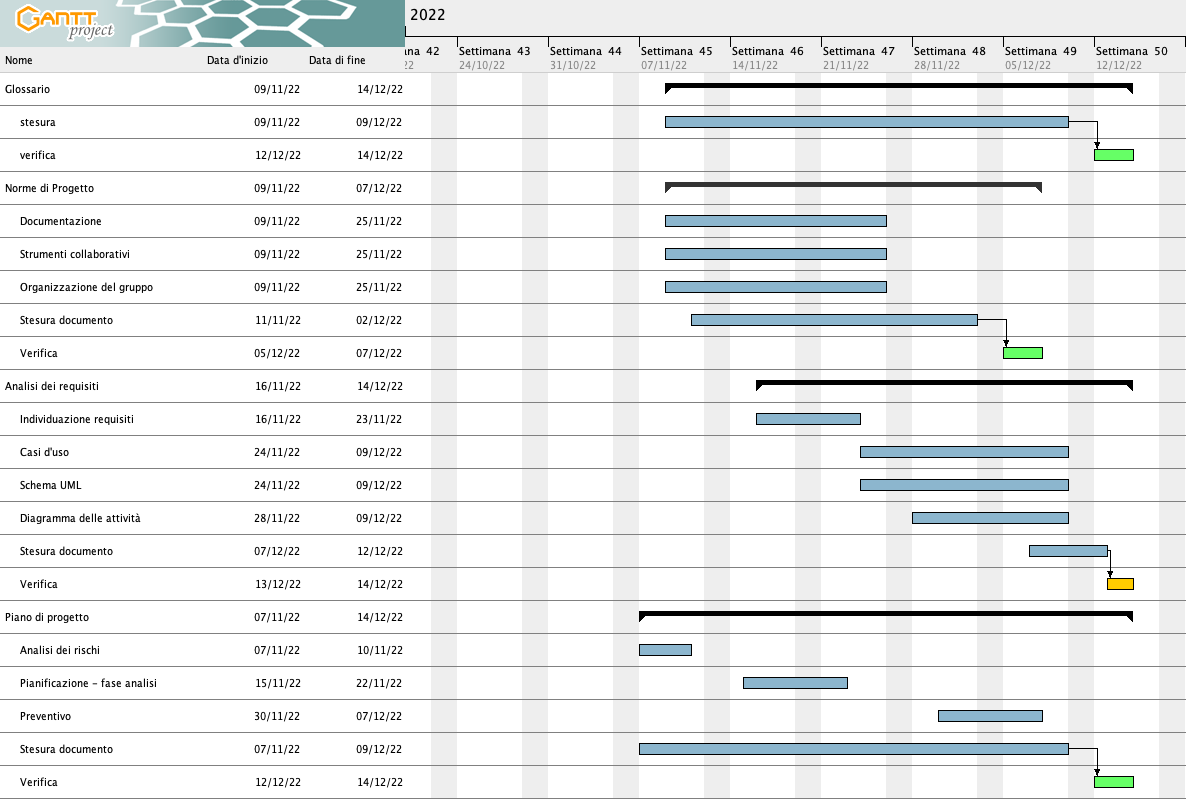
\includegraphics[scale=0.38]{image/analisi_preliminare_gantt.png}
    \caption{Diagramma di Gantt\textsubscript{g} fase di Analisi preliminare}
\end{figure}
\pagebreak
%fase Poc\textsubscript{g}

\subsection{Progettazione Proof of Concept\textsubscript{g}}
Questo periodo comincia al termine del periodo di Analisi preliminare e termina con l'inizio della codifica del Proof of Concept\textsubscript{g}.\\
\begin{center}
\textbf{periodo:} dal 15-12-2022 al 16-01-2023\\
\end{center}
Questo periodo viene dedicato al completamento delle attività arretrate, per poi concentrarsi sulla 
progettazione e iniziare la codifica del Proof of Concept\textsubscript{g}. Si va inoltre avanti con la stesura 
della documentazione. Questo periodo viene suddiviso nelle attività trattate nella seguente sezione.

\subsubsection{Attività}
\begin{itemize}
\item \textbf{\textit{Glossario}:} il documento viene costantemente aggiornato con nuovi termini;
\item \textbf{\textit{Piano di Progetto}:} viene aggiunta la pianificazione del periodo, il preventivo e il consultivo;  
\item \textbf{Analisi dei requisti:} si continua la stesura del documento, completando le attività arretrate dal periodo precedente;
\item \textbf{\textit{Piano di Qualifica}:} documento nel quale vengono stabiliti gli standard di qualità di processo\textsubscript{g} e di prodotto\textsubscript{g};
\item \textbf{\textit{Norme di Progetto}:} vengono aggiunte nuove norme relative alla documentazione e alle metriche utilizzate nel \textit{Piano di Qualifica};
\item \textbf{Proof of Concept\textsubscript{g}:} ogni componente del gruppo studierà individualmente le tecnologie da utilizzare, per prendere familliarità; si inizierà poi a progettare e realizzare il Proof of Concept\textsubscript{g}, una versione semplice, ma dimostrativa, del prodotto\textsubscript{g} finale, per 
capire se è fattibile e darne una prova al proponente\textsubscript{g}.
\end{itemize}

\subsubsection{Periodi}
La Progettazione Proof of concept\textsubscript{g} sarà suddivisa nei seguenti periodi:
\begin{itemize}
\item \textbf{Periodo 1:} \textit{dal 15-12-2022 al 21-12-2022}, pianificazione del periodo corrente con relativo preventivo, completamento attività arretrate 
(stesura del documento \textit{Analisi dei Requisiti}). Continua lo studio individuale delle tecnologie da utilizzare;
\item \textbf{Periodo 2:} \textit{dal 22-12-2022 al 04-01-2023}, inizia la stesura del documento \textit{Piano di Qualifica}. Inizia la progettazione del Proof of Concept\textsubscript{g}, si continua la stesura e la verifica\textsubscript{g} dei documenti;
\item \textbf{Periodo 3:} \textit{dal 05-01-2023 al 16-01-2023}, continua la progettazione e inizia la codifica del Proof of Concept\textsubscript{g}. Si procede nella stesura e nella verifica\textsubscript{g} della documentazione.
\end{itemize}

\begin{figure}[H]
    \centering
    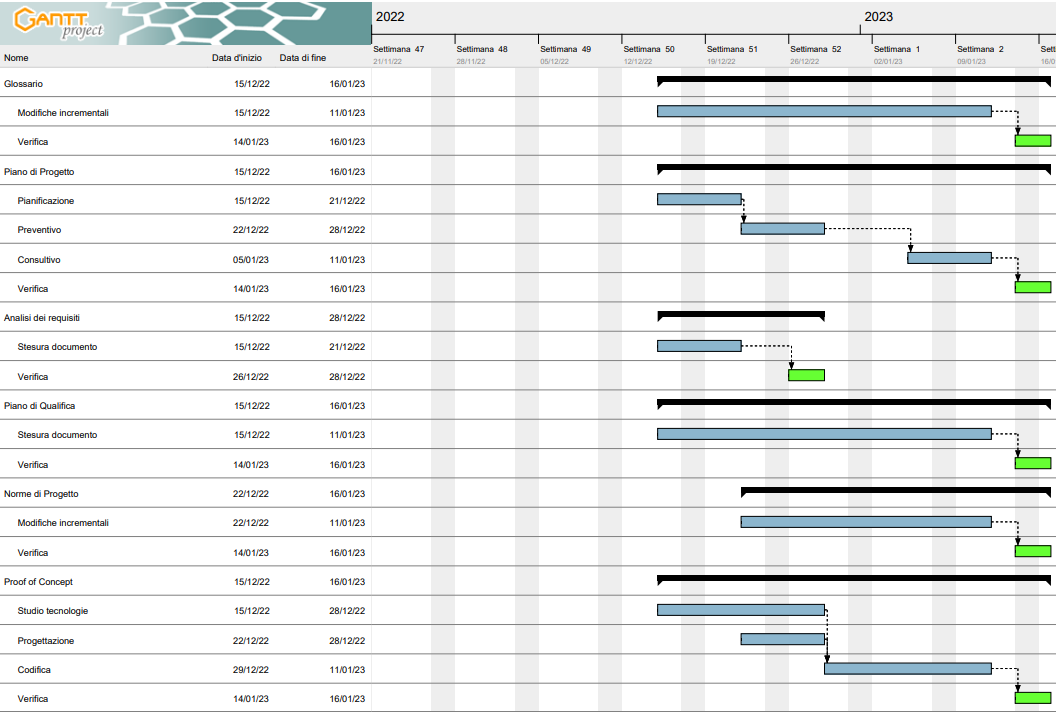
\includegraphics[scale=0.72]{image/gantt_poc.png}
    \caption{Diagramma di Gantt\textsubscript{g} fase di Progettazione Proof of Concept\textsubscript{g}}
\end{figure}
\pagebreak

\subsection{Codifica Proof of Concept\textsubscript{g}}
Questo periodo comincia al termine del periodo di Progettazione Proof of Concept\textsubscript{g} e termina con 
la consegna dei documenti per la Requirements and Tecnology Baseline.\\
\begin{center}
\textbf{periodo:} dal 17-01-2023 al 15-02-2023\\
\end{center}
In questo periodo ci si concentra sul portare a termine la codifica del Proof of Concept\textsubscript{g}, viene completata la stesura della documentazione, che 
viene alla fine approvata per la RTB. 

\subsubsection{Attività}
\begin{itemize}
\item \textbf{\textit{Glossario}:} il documento viene costantemente aggiornato con nuovi termini;
\item \textbf{\textit{Piano di Progetto}:} viene aggiunta la pianificazione del periodo, il preventivo e il consultivo;  
\item \textbf{Analisi dei Requisti:} si termina la stesura del documento applicando le modifiche necessarie;
\item \textbf{\textit{Piano di Qualifica}:} si continua con la stesura del documento;
\item \textbf{\textit{Norme di Progetto}:} viene cambiato l'indice del documento per avere una conformità con il \textit{Piano di Qualifica}, 
si completa la stesura delle sezioni mancanti;
\item \textbf{Proof of Concept\textsubscript{g}:} si completa la codifica del PoC\textsubscript{g}, aggiungendo le funzionalità stabilite in accordo con il proponente\textsubscript{g}.
\end{itemize}

\subsubsection{Periodi}
Il periodo di Codifica Proof of Concept\textsubscript{g} sarà suddivisa nei seguenti periodi:
\begin{itemize}
\item \textbf{Periodo 1:} \textit{dal 17-01-2023 al 31-01-2023}, pianificazione del periodo corrente con relativo preventivo, si continua la codifica 
del Proof of Concept\textsubscript{g}. Prosegue la stesura del \textit{Piano di Qualifica} aggiornando le metriche da seguire; si aggiornano le \textit{Norme di Progetto} di conseguenza;
\item \textbf{Periodo 2:} \textit{dal 01-02-2023 al 15-02-2023},  viene completata la codifica del PoC\textsubscript{g} e la stesura della documentazione. 
Si verifica\textsubscript{g} nel \textit{Piano di Qualifica} che le metriche siano rispettate. Si verificano e approvano tutti i documenti in previsione della RTB.
\end{itemize}

\begin{figure}[H]
    \centering
    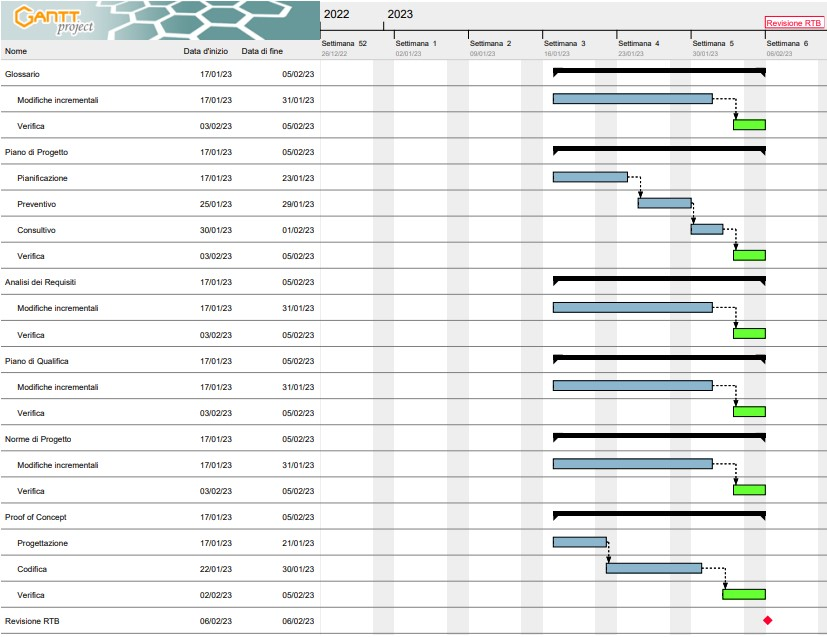
\includegraphics[scale=0.56]{image/gantt_terzo_periodo.png}
    \caption{Diagramma di Gantt\textsubscript{g} fase di Codifica Proof of concept\textsubscript{g}}
\end{figure}
\pagebreak

\pagebreak
\input{res/sections/04_Preventivo.tex}
\pagebreak
\section{Consuntivo}
%introduzione
\subsection{Introduzione}
Questa sezione riporta i dati raccolti durante il progetto riguardo le ripartizioni dei ruoli e le ore impiegate da parte di tutti i componenti del gruppo e viene posta in confronto alle previsioni pianificate nella sezione di consuntivo.

%qui verrà inserito il consuntivo finale con tutte le ore del progetto.

\subsection{Dettaglio periodi}
In questa sezione viene mostrato l'effettivo utilizzo di ore per ogni componente del gruppo, calcolato alla fine di ogni fase del progetto.

\subsubsection{Analisi Preliminare}
Qui di seguito riportiamo la suddivisione dei ruoli e le ore di lavoro effettive impiegate nel periodo di Analisi Preliminare:

\begin{longtable}{ 
	>{\centering}M{0.15\textwidth} 
	>{\centering}M{0.075\textwidth}
	>{\centering}M{0.085\textwidth}
	>{\centering}M{0.075\textwidth}
	>{\centering}M{0.075\textwidth}
	>{\centering}M{0.095\textwidth}
	>{\centering}M{0.075\textwidth}
	>{\centering}M{0.085\textwidth}
	>{\centering\arraybackslash}M{0.06\textwidth} 
	}
	\rowcolorhead
	\centering \headertitle{Ruolo} &
	\headertitle{Marco} &	
	\headertitle{Giacomo} &
	\headertitle{Elena} &
	\headertitle{Mirko} &
	\headertitle{Tommaso} &
	\headertitle{Rino} &
	\headertitle{Gabriele} &
	\headertitle{Totale}
	\endfirsthead	
	\endhead
	
	Responsabile & 10 (-1) & - & 8 & - & 8 & - & - & 25 \tabularnewline
	Amministratore & - & -  & - & - & 9 (-1) & 9 & - & 17 \tabularnewline
	Analista & 13 (-2)& 11 (-1)  & 15(-2) & 12 & - & 14(-1) & 12 & 71 \tabularnewline
	Progettista & - & -  & - & - & - & - & - & 0 \tabularnewline
	Programmatore & - & - & - & - & - & - & - & 0 \tabularnewline
	Verificatore & - & 15 (+1) & - & 13 & 11 (+1) & - & 13 (+1) & 55 \tabularnewline
	\rowcolorhead \textcolor{white}{\textbf{Totale}} & \textcolor{white}{\textbf{20}} &\textcolor{white}{\textbf{26}} & \textcolor{white}{\textbf{21}} & \textcolor{white}   {\textbf{25}} & 	\textcolor{white}{\textbf{28}} & \textcolor{white}{\textbf{22}} & \textcolor{white}{\textbf{26}} & 	\textcolor{white}{\textbf{168}}\\
		\captionline\caption{Rendiconto effettivo della distribuzione delle ore nel periodo di Analisi Preliminare}
\end{longtable}

I costi effettivi del periodo sono i seguenti:

\begin{longtable}{
	>{\centering}M{0.25\textwidth} 
	>{\centering}M{0.10\textwidth}
	>{\centering\arraybackslash}M{0.15\textwidth} 
	}
	\rowcolorhead
	\centering \headertitle{Ruolo} &
	\headertitle{Ore} &	
	\headertitle{Costo}
	\endfirsthead
	\endhead
	
	Responsabile & 26(-1) & 780(-30)€  \tabularnewline
	Amministratore & 18(-1)  & 360(-20)€  \tabularnewline
	Analista & 77(-6)  & 1925(-150)€  \tabularnewline
	Progettista & 0  & 0  \tabularnewline
	Programmatore & 0 & 0  \tabularnewline
	Verificatore & 52(+3) & 780(+45)€ \tabularnewline
	\rowcolorhead \textcolor{white}{\textbf{Totale Consuntivo}} &\textcolor{white}{\textbf{168}}& \textcolor{white}{\textbf{3090€}}	\\
	\rowcolorhead \textcolor{white}{\textbf{Totale Preventivo}} &\textcolor{white}{\textbf{175}}& \textcolor{white}{\textbf{3245€}}	\\
	\rowcolorhead \textcolor{white}{\textbf{Differenza}} &\textcolor{white}{\textbf{-7}}& \textcolor{white}{\textbf{-155€}}	\\
	\captionline\caption{Prospetto costi nel periodo di Analisi Preliminare} 

\end{longtable}

\paragraph{Resoconto}
\begin{itemize}
	\item \textbf{Analista (-6 ore)}: a causa dell'inesperienza non è stato calcolato accuratamente il 
	tempo necessario per svolgere le attività degli analisti;
	\item \textbf{Verificatore (+3 ore)}: le attività dei verificatori si sono rivelate più lunghe in termini di tempi di lavoro. 
	Per questo motivo sono state impiegate più ore del previsto.  
\end{itemize}
In generale il gruppo ha impiegato meno ore di quelle preventivate, non riuscendo a 
terminare tutte le attività previste. Sono stati sottovalutati i tempi di verifica\textsubscript{g}, che risultano essere più lunghi 
del previsto. Il bilancio è positivo, ma è necessaria una ripianificazione per completare le attività rimaste indietro.


\subsubsection{Progettazione Proof of Concept\textsubscript{g}}
Qui di seguito riportiamo la suddivisione dei ruoli e le ore di lavoro effettive impiegate per la fase di Progettazione Proof of Concept\textsubscript{g}:

\begin{longtable}{ 
	>{\centering}M{0.20\textwidth} 
	>{\centering}M{0.06\textwidth}
	>{\centering}M{0.10\textwidth}
	>{\centering}M{0.05\textwidth}
	>{\centering}M{0.06\textwidth}
	>{\centering}M{0.10\textwidth}
	>{\centering}M{0.05\textwidth}
	>{\centering}M{0.09\textwidth}
	>{\centering\arraybackslash}M{0.06\textwidth} 
	}
	\rowcolorhead
	\centering \headertitle{Ruolo} &
	\headertitle{Marco} &	
	\headertitle{Giacomo} &
	\headertitle{Elena} &
	\headertitle{Mirko} &
	\headertitle{Tommaso} &
	\headertitle{Rino} &
	\headertitle{Gabriele} &
	\headertitle{Totale}
	\endfirsthead	
	\endhead
	
	Responsabile & - & - & - & 12 & - & - & - & 12 \tabularnewline
	Amministratore & - & -  & - & - & - & - & - & 0 \tabularnewline
	Analista & -  & -  & - & - & 12 & - & - & 12 \tabularnewline
	Progettista & 3 (+1) & 9  (-2) & - & - & 3 & 6 & 7 & 27 \tabularnewline
	Programmatore & 5 & 15 & 9 (+1) & 8 & - & 16 & 16 (-2) & 68 \tabularnewline
	Verificatore & 14 (-2) & - & 12 (-2) & - & 5 & - & - & 27 \tabularnewline
	\rowcolorhead \textcolor{white}{\textbf{Totale}} & \textcolor{white}{\textbf{21}} &\textcolor{white}{\textbf{22}} & \textcolor{white}{\textbf{20}} & \textcolor{white}{\textbf{20}} & 	\textcolor{white}{\textbf{20}} & \textcolor{white}{\textbf{22}} & \textcolor{white}{\textbf{21}} & 	\textcolor{white}{\textbf{146}}\\
	\captionline\caption{Rendiconto effettivo della distribuzione delle ore nel periodo di Progettazione Proof of Concept\textsubscript{g}}
\end{longtable}

I costi effettivi del periodo sono i seguenti:

\begin{longtable}{ 
		>{\centering}M{0.25\textwidth} 
		>{\centering}M{0.10\textwidth}
		>{\centering\arraybackslash}M{0.15\textwidth} 
		}
	\rowcolorhead
	\headertitle{Ruolo} &
	\headertitle{Ore} &
	\headertitle{Costo} 
	\endfirsthead	
	\endhead
	
	Responsabile & 12  & 360\euro\tabularnewline
	Amministratore & 0 & 0\euro \tabularnewline
	Analista & 12 & 300\euro \tabularnewline
	Progettista & 27 (-1) & 700(-25)\euro \tabularnewline
	Programmatore & 68 (-1) & 1035(-15)\euro \tabularnewline
	Verificatore & 27 (-4) & 465(-60)\euro \tabularnewline
	\rowcolorhead \textcolor{white}{\textbf{Totale Consuntivo}} & \textcolor{white}{\textbf{146}} & \textcolor{white}{\textbf{2760\euro}}\\
	\rowcolorhead \textcolor{white}{\textbf{Totale Preventivo}} & \textcolor{white}{\textbf{152}} & \textcolor{white}{\textbf{2860\euro}}\\
	\rowcolorhead \textcolor{white}{\textbf{Differenza}} & \textcolor{white}{\textbf{-6}} & \textcolor{white}{\textbf{-100\euro}}\\
	\captionline\caption{Prospetto costi nel periodo di Progettazione Proof of Concept\textsubscript{g}} 
\end{longtable}

\paragraph{Resoconto}
In questo periodo il gruppo non è riuscito a rispettare pienamente quanto previsto dal preventivo. Si 
è verificato un rallentamento nei ritmi di lavoro, che, se pur preso in considerazione nel preventivo, ha causato comunque 
una riduzione delle ore complessive di lavoro e della spesa totale. Le cause di questo rallentamento sono state individuate in:
\begin{itemize}
	\item Presenza di festività;
	\item Impegni personali;
	\item Alcuni componenti del gruppo sono stati impegnati più 
	del necessario a causa della sessione di esami.
\end{itemize}
Il gruppo è comunque riuscito a completare tutte le attività previste e a svolgere un incontro 
con il proponente\textsubscript{g}, ottenendo un feedback sul lavoro svolto e ulteriori indicazioni da seguire.
Per migliorare l'accuratezza dei preventivi si è deciso di tenere in maggiore considerazione gli impegni di ogni 
componente del gruppo e l'impatto che essi hanno di conseguenza sul lavoro cooperativo.


\subsubsection{Codifica Proof of Concept\textsubscript{g}}
Qui di seguito riportiamo la suddivisione dei ruoli e le ore di lavoro effettive impiegate per la fase di Codifica Proof of Concept\textsubscript{g}:

\begin{longtable}{ 
	>{\centering}M{0.20\textwidth} 
	>{\centering}M{0.06\textwidth}
	>{\centering}M{0.10\textwidth}
	>{\centering}M{0.05\textwidth}
	>{\centering}M{0.06\textwidth}
	>{\centering}M{0.10\textwidth}
	>{\centering}M{0.05\textwidth}
	>{\centering}M{0.09\textwidth}
	>{\centering\arraybackslash}M{0.06\textwidth} 
	}
	\rowcolorhead
	\centering \headertitle{Ruolo} &
	\headertitle{Marco} &	
	\headertitle{Giacomo} &
	\headertitle{Elena} &
	\headertitle{Mirko} &
	\headertitle{Tommaso} &
	\headertitle{Rino} &
	\headertitle{Gabriele} &
	\headertitle{Totale}
	\endfirsthead	
	\endhead
	
	Responsabile & - & - & - & 4 & - & - & 4 & 8 \tabularnewline
	Amministratore & - & -  & - & - & - & - & - & 0 \tabularnewline
	Analista & -  & -  & - & - & 8 (-1) & - & - & 7 \tabularnewline
	Progettista & - & 3 & - & - & - & 2 & 3 (-1) & 7 \tabularnewline
	Programmatore & - & 8 (+2) & - & 5 & - & 13 (+1) & 7 & 36 \tabularnewline
	Verificatore & 12 (-1) & - & 13 & 5 & 4(-1) & - & - & 32 \tabularnewline
	\rowcolorhead \textcolor{white}{\textbf{Totale}} & \textcolor{white}{\textbf{11}} &\textcolor{white}{\textbf{13}} & \textcolor{white}{\textbf{13}} & \textcolor{white}{\textbf{14}} & 	\textcolor{white}{\textbf{10}} & \textcolor{white}{\textbf{16}} & \textcolor{white}{\textbf{13}} & 	\textcolor{white}{\textbf{90}}\\
	\captionline\caption{Rendiconto effettivo della distribuzione delle ore nel periodo di Codifica Proof of Concept\textsubscript{g}}
\end{longtable}

I costi effettivi del periodo sono i seguenti:

\begin{longtable}{ 
		>{\centering}M{0.25\textwidth} 
		>{\centering}M{0.10\textwidth}
		>{\centering\arraybackslash}M{0.15\textwidth} 
		}
	\rowcolorhead
	\headertitle{Ruolo} &
	\headertitle{Ore} &
	\headertitle{Costo} 
	\endfirsthead	
	\endhead
	
	Responsabile & 8  & 240\euro\tabularnewline
	Amministratore & 0 & 0\euro \tabularnewline
	Analista & 7 (-1) & 200(-25)\euro \tabularnewline
	Progettista & 7 (-1) & 200(-25)\euro \tabularnewline
	Programmatore & 36 (+3) & 495(+45)\euro \tabularnewline
	Verificatore & 32 (-2) & 510(-30)\euro \tabularnewline
	\rowcolorhead \textcolor{white}{\textbf{Totale Consuntivo}} & \textcolor{white}{\textbf{90}} & \textcolor{white}{\textbf{1610\euro}}\\
	\rowcolorhead \textcolor{white}{\textbf{Totale Preventivo}} & \textcolor{white}{\textbf{91}} & \textcolor{white}{\textbf{1645\euro}}\\
	\rowcolorhead \textcolor{white}{\textbf{Differenza}} & \textcolor{white}{\textbf{-1}} & \textcolor{white}{\textbf{-35\euro}}\\
	\captionline\caption{Prospetto costi nel periodo di Codifica Proof of Concept\textsubscript{g}} 
\end{longtable}

\paragraph{Resoconto}
\begin{itemize}
	\item \textbf{Programmatore (+3 ore)}: nella codifica del Proof of Concept\textsubscript{g} sono state necessarie più 
	ore di lavoro del previsto a causa della poca familiarità che il gruppo aveva con le tecnologie scelte;
	\item \textbf{Verificatore (-2 ore)}: le attività dei verificatori hanno richiesto meno tempo del previsto.  
\end{itemize}
Nonostante alcune discrepanze nei singoli ruoli, in totale le ore effettive risultano in linea con 
quelle preventivate, con una differenza di costi di 35\euro.

\pagebreak
\section{Attualizzazione dei rischi}
In questa sezione sono riportati i rischi che si sono verificati durante il corso del progetto e 
le misure di mitigazione che il gruppo ha attuato di conseguenza.
\subsection{Analisi Preliminare}
\begin{longtable}{ 
	>{\centering}M{0.20\textwidth} 
	>{\raggedright}M{0.30\textwidth}
	>{\raggedright}M{0.40\textwidth}
	}
	\rowcolorhead
	\centering 
	\headertitle{Nome} &	
	\headertitle{Descrizione} &
	\headertitle{Mitigazione}
	\endfirsthead	
	\endhead
	
	\textbf{Inesperienza tecnologica} & 
    Alcuni componenti del gruppo hanno trovato difficolta nell'utilizzo di GitHub\textsubscript{g}. & 
    Si sono svolte delle riunioni in cui i componenti più esperti nell'utilizzo di GitHub\textsubscript{g} 
    hanno spiegato le basi e aiutato i componenti più in difficoltà.  \tabularnewline
    \textbf{Pianificazione inadeguata} & Sono state preventivate troppe ore di 
    lavoro rispetto a quelle che il gruppo era effettivamente in grado di svolgere. Non tutte le 
    attività previste sono quindi state portate a termine.  & 
    Si è cercato di ripianificare con maggiore precisione, senza sovrastimare il tempo disponibile dei 
    componenti del gruppo. \tabularnewline
    \textbf{Comprensione dei requisiti} & Alcuni requisiti non sono stati compresi subito a pieno dal gruppo.  & 
    Si è contattato il proponente\textsubscript{g} per un chiarimento immediato dei dubbi. \tabularnewline
	\captionline \caption{Attualizzazione dei rischi nel periodo di Analisi preliminare}
\end{longtable}

\subsection{Progettazione Proof of Concept\textsubscript{g}}
\begin{longtable}{ 
	>{\centering}M{0.20\textwidth} 
	>{\raggedright}M{0.30\textwidth}
	>{\raggedright}M{0.40\textwidth}
	}
	\rowcolorhead
	\centering 
	\headertitle{Nome} &	
	\headertitle{Descrizione} &
	\headertitle{Mitigazione}
	\endfirsthead	
	\endhead
	
	\textbf{Disponibilità dei componenti} & 
    A causa delle festività e della sessione di esami la disponibilità dei componenti del gruppo 
    si è ridotta. & 
    Nella pianificazione del periodo si è tenuto conto di questi possibili rallentamenti.  \tabularnewline
	\captionline \caption{Attualizzazione dei rischi nel periodo di Progettazione Proof of Concept\textsubscript{g}}
\end{longtable}

\subsection{Codifica Proof of Concept\textsubscript{g}}
\begin{longtable}{ 
	>{\centering}M{0.20\textwidth} 
	>{\raggedright}M{0.30\textwidth}
	>{\raggedright}M{0.40\textwidth}
	}
	\rowcolorhead
	\centering 
	\headertitle{Nome} &	
	\headertitle{Descrizione} &
	\headertitle{Mitigazione}
	\endfirsthead	
	\endhead
	
	\textbf{Inesperienza tecnologica} & 
    Durante la codifica del PoC\textsubscript{g} sono sorte alcune difficoltà a causa della poca
    familiarità da parte del gruppo sulle tecnologie da utilizzare. & 
    C'è stato un periodo di studio individuale delle tecnologie per acquisire maggiore padronanza. 
    Tutti si sono impegnati ad aiutarsi a vicenda all'insorgere di problemi. \tabularnewline
	\captionline \caption{Attualizzazione dei rischi nel periodo di Codifica Proof of Concept\textsubscript{g}}
\end{longtable}
\pagebreak
\end{document}
